\documentclass{article}
\usepackage{booktabs}
\usepackage{fancyhdr}
\pagestyle{empty}
\usepackage{graphicx}
 \usepackage{color}
 \usepackage{transparent}
 \usepackage{hyperref}
 \usepackage{lastpage}

\pagestyle{fancy}
\lhead{} % Top left header
\chead{Heqet Application Report} % Top center head
\rhead{} % Top right header
\lfoot{} % Bottom left footer
\cfoot{} % Bottom center footer
\rfoot{ \thepage/\protect\pageref{LastPage}} % Bottom right footer \protect\pageref{LastPage}

\newcommand{\prob}[1]{\noindent\textbf{#1.}}

\begin{document}
\pagestyle{empty}
\begin{center}
\vspace{3cm}
\scalebox{1.5}{{\Huge Heqet Application Report}}

\vspace{2cm}
{\Large By Isaac Reilly}

\vspace{0.15cm}
{\large advised by Donya Quick}

\vspace{0.1cm}
{continuation of my senior project for the Yale University major in Computer Science}

\vspace{13cm}

{\small spring 2016}

\end{center}

\pagebreak
\pagestyle{plain}

%\tableofcontents
%\newpage

\begin{section}{Overview}
Last semester, I created the Heqet library to improve music representation and manipulation in Haskell and to export Lilypond code to make pleasing printed scores. My project this semester was to create a graphical application using the Heqet library, with some additional features like multiple selections and a automatically updating dependency graph. 

\end{section}
\begin{section}{How did it turn out?}
The project turned out to be vastly more than I could finish in a semester, but my efforts have laid a solid foundation for future work. The graphical interface, which I built using the \texttt{threepenny-gui} library, is almost complete and includes navigation, music rendering, and many palettes of buttons. Rendering the music in real time turned out to be an issue: I was hoping to use an speed-optimized form of Lilypond, but this proved impossible. Instead, I created a fast music drawing system which avoided many aesthetic adjustments of the output which slow down Lilypond, such as varying the horizontal spacing of notes.

I adapted the Heqet library for the application and converted it to use the Stack build system for Haskell rather than Cabal. The Heqet library still needs some work, such as implementing dynamics and polishing the time signature handling.

As predicted, the bulk of my work was on the application. I spun off the library for the dependency graph and undo into the \texttt{history-graph} library and built the framework for almost the whole application. I wish to emphasize that although the application is not usable, the code is in a much better state than it may seem. I have solved most of the hard problems of the project, but I ran out of time to implement the easy stuff. For example, many of the editing functions corresponding to currently-nonfunctional buttons are trivial to implement. A more complicated example: there is no ability to open or save files, but an important design point, the function ``registry'', provides the ability to encode history actions as text, since functions themselves can't be easily stored in a file. The functional reactive programming UI framework should make it straightforward to add the click-to-select functionality.

\end{section}
\begin{section}{What I Learned}

As in last semester, I've grown in my ability to find satisfaction in a large project that is not complete. I have some time off this summer before starting to work full-time, and I am very excited to continue with Heqet and make it available to users.

My skills in Haskell programming and software architecture have improved, particularly when I studied functional reactive programming.

\end{section}
\begin{section}{Haskell}

The Haskell language continues to live up to its reputation: I had almost no semantic bugs once clearing the type errors, and refactoring, such as when I added the function registry, went smoothly. My  attempts to change the structure of the Heqet library's music representation didn't go well, but that was due to problems with my algorithms which would have necessitated a large refactoring that I decided to forgo in favor of focusing on the application. I didn't know what to expect from functional reactive programming, but it turned out to be simple and concise.
\end{section}

\begin{section}{Future Goals}

I now have even more open issues on Heqet's GitHub tracker: 149. In addition to the features I haven't yet implemented, there are more improvements I would like to make, such as prettier drawn music on the real-time canvas and support for multiple music notation systems, such as a text-based display suitable for screenreaders, braille music in a format for a tactile display, early music notation, and a notation system of my own design. I plan to make complete builds available for a variety of systems. I look forward to continuing with this project!

\end{section}


\begin{section}{Images}
The empty screen:

\hspace{-1.5cm}\scalebox{0.3}{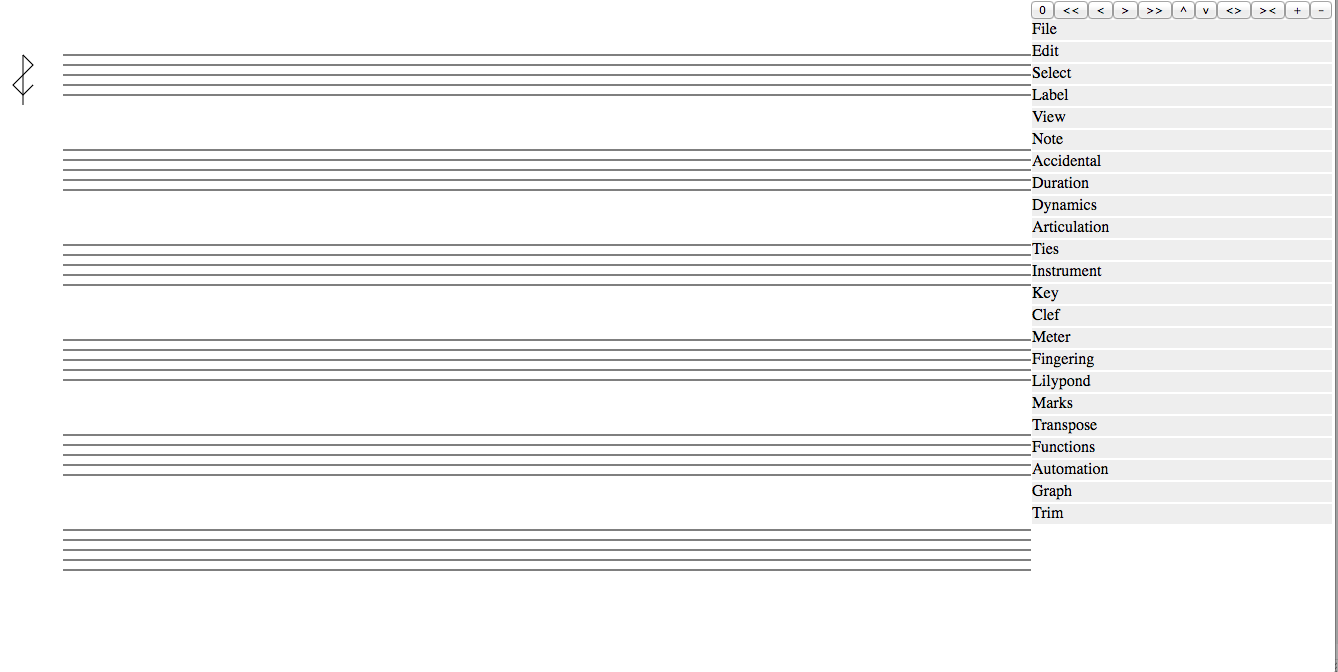
\includegraphics{app-full}}

\pagebreak
The menus on the right side, expanded:

\hspace{-0.8cm}\scalebox{0.4}{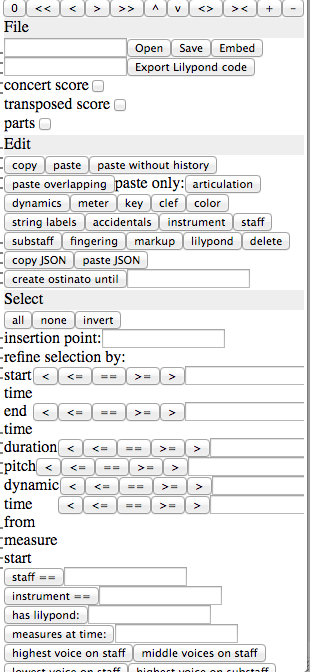
\includegraphics{interface1} }
\hspace{1mm}\scalebox{0.4}{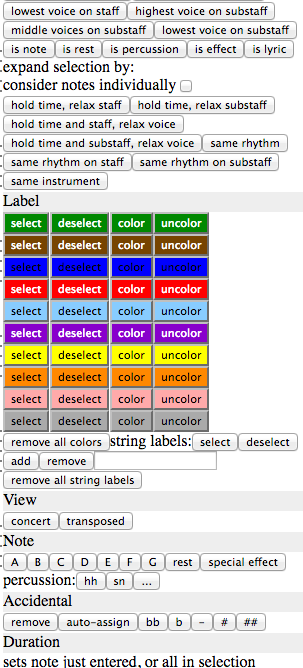
\includegraphics{interface2}}
\hspace{1mm}\scalebox{0.4}{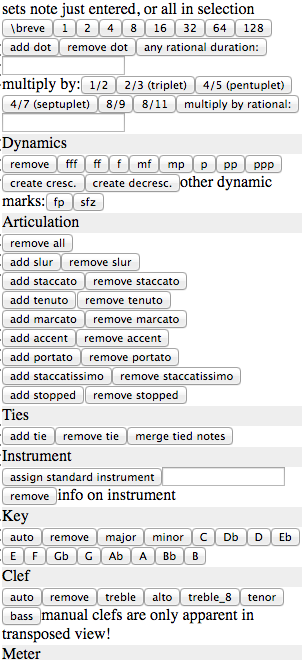
\includegraphics{interface3}}
\scalebox{0.4}{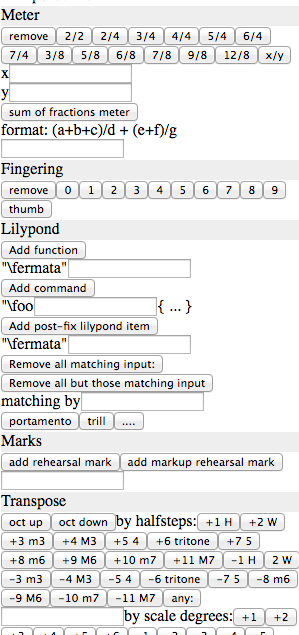
\includegraphics{interface4}}
\hspace{1mm}\scalebox{0.4}{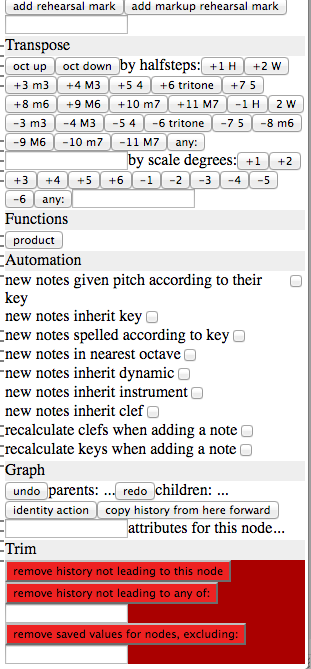
\includegraphics{interface5}}

\vspace{1cm}
A demonstration of various glyphs:

\hspace{-1.5cm}\scalebox{0.4}{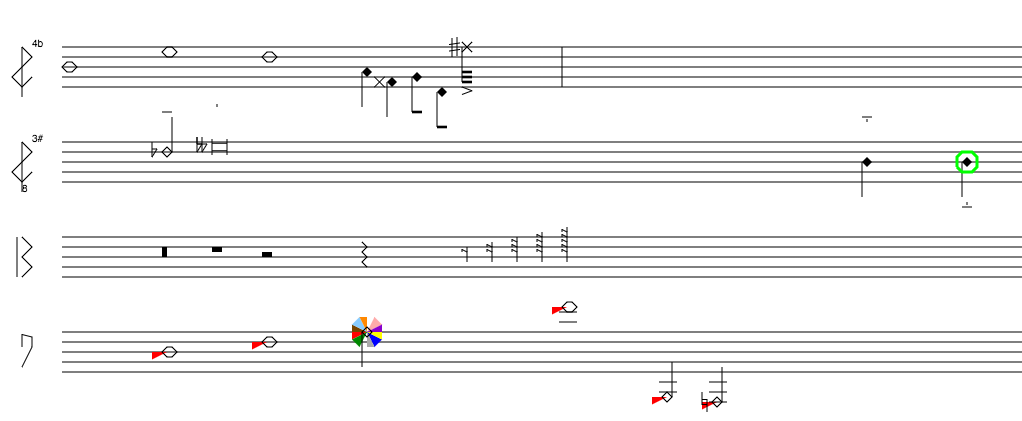
\includegraphics{notes}}

\end{section}

\end{document}